\documentclass{article}
\usepackage{graphicx}
\usepackage{amsmath}
\usepackage{float}
\usepackage{amsfonts}
\usepackage{listings}
\usepackage{xcolor}
\usepackage[utf8]{inputenc}
\usepackage{hyperref}
\usepackage{fancybox}
\usepackage{booktabs}
\usepackage{tikz}
\usepackage[margin=2cm]{geometry}
\usetikzlibrary{shapes, arrows.meta, positioning}
\usepackage[labelfont=bf, font=small]{caption}  % Pour personnaliser le titre de la figure


\lstset{
  language=R,
  basicstyle=\ttfamily\small,
  numbers=left,               % Numérotation des lignes
  numberstyle=\tiny\color{gray}, % Style de la numérotation
  keywordstyle=\color{blue},  % Couleur des mots-clés
  commentstyle=\color{green}, % Couleur des commentaires
  stringstyle=\color{red},    % Couleur des chaînes de caractères
  breaklines=true,            % Coupe les lignes trop longues
  frame=single,               % Encadre le code
}


\title{TP1 TID}
\author{SCAIA Matteo, MARIAC Damien}
\date{\today} 

\begin{document}

\maketitle

\begin{figure}[h] 
    \centering
    
\includegraphics[width=0.5\textwidth]{ssd_logo.png} 
\end{figure}

\begin{figure}[h] 
    \centering
    
\includegraphics[width=0.5\textwidth]{logo_um_2022_rouge_RVB.png} 
\end{figure}

\newpage

\tableofcontents

\newpage

\section{Exercice 1}
On considère le tableau ci-dessous, répartissant la population active occupée selon l'âge ($A$), le sexe ($S$) et la
catégorie socioprofessionnelle ($C$) (source: INSEE, enquête emploi 2016).
\begin{figure}[ht]
  \centering
  \setlength{\fboxsep}{0pt}  % Pour que l'image soit bien ajustée dans le cadre
  \setlength{\fboxrule}{1pt}  % Épaisseur du cadre
  \fbox{%
    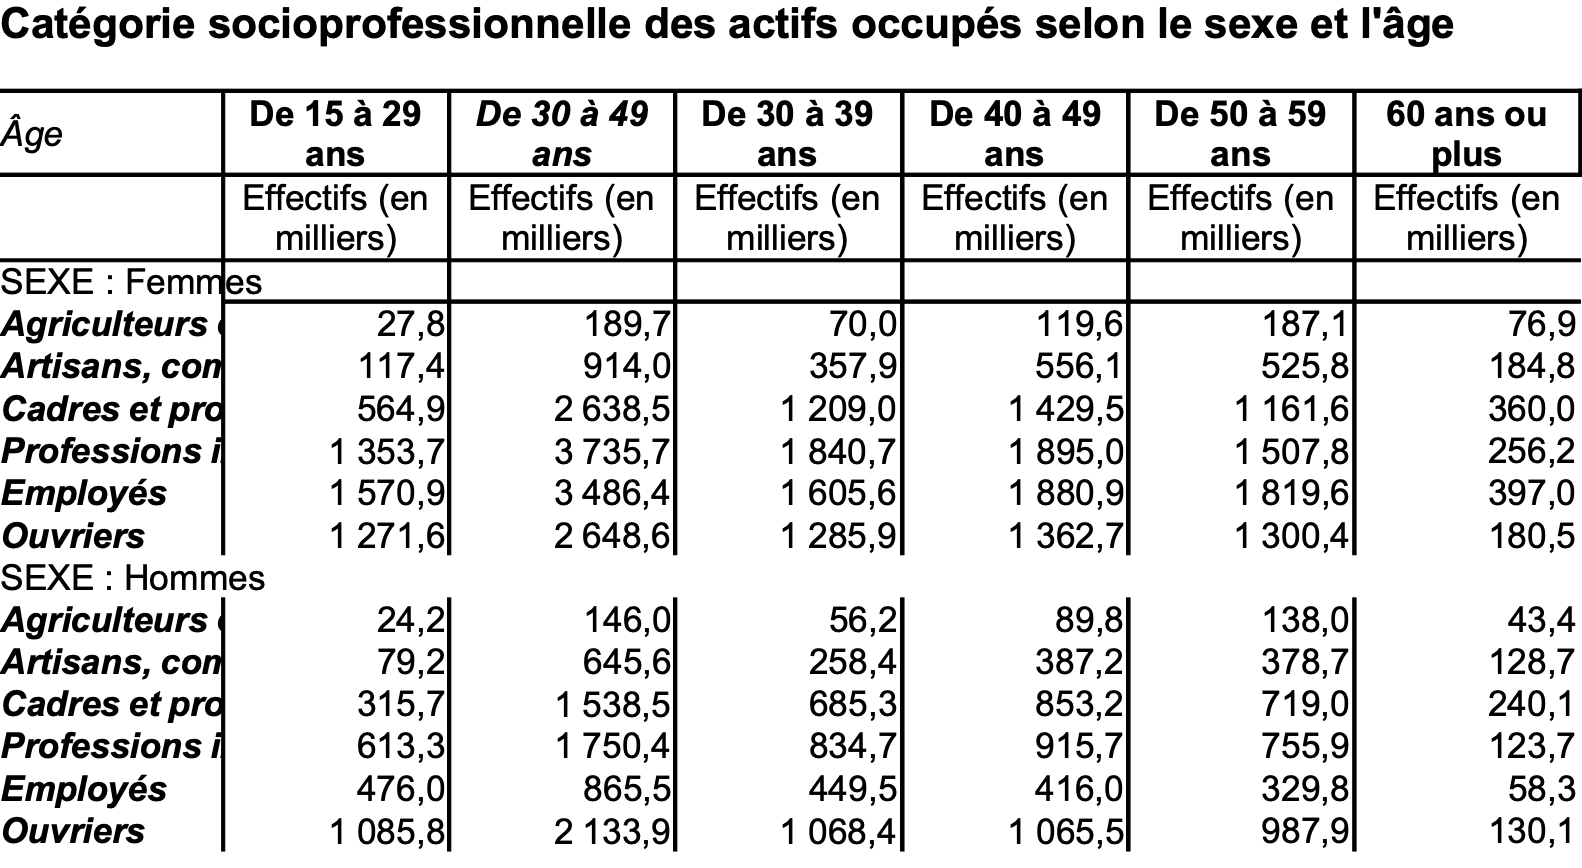
\includegraphics[width=0.7\textwidth]{CE.png}
  }
  \caption{Tableau répartissant la population active occupée selon des catégories }
\end{figure}
\subsection{Modélisation et variable}
\label{1.1}
Tout d'abord de manière intuitive, nous avons envie de modéliser la variable
socioprofessionnelle avec les deux autres. Cependant, nous devons
le montrer de manière formelle. Grâce au code fourni dans la partie \ref{sec : Annexe},
nous calculons l'information mutuelle de chacune des variables.\\\\
Premièrement, nous calculons l'entropie de chacune de ces variables.\\
Pour la variable $A$, nous avons le tableau suivant (en fréquence). 
\begin{table}[ht]
  \centering
  \begin{tabular}{|l|l|l|l|l|l|l|}
    \hline
    & 15-29 ans  & 30-39 ans  & 40-49 ans  & 50-59 ans  & 60+ ans \\ \hline
    Age & 0.1866 & 0.2419 & 0.2730 & 0.2441 & 0.0542 \\ \hline
  \end{tabular}
  \caption{Distribution par âge ($A$)}
\end{table}
\\Nous pouvons calculer l'entropie de $A$.\\
\[
H(A) = -\sum_{n = 1}^{6}p_i\log_2(p_i)=2,1833
\]
De même manière, nous calculons l'entropie de $C$ et $S$.\\
\begin{table}[H]
  \centering
  \begin{tabular}{|l|l|l|}
  \hline
             & Femme  & Homme  \\ \hline
  Proportion & 0,6589 & 0,3411 \\ \hline
  \end{tabular}
  \caption{Distribution par sexe ($S$)}
\end{table}

\begin{table}[H]
  \centering
  \begin{tabular}{|l|l|l|l|l|l|l|}
  \hline
             & Agriculteur & Artisans & Cadres & Profession In & Employes & Ouvrier \\ \hline
  Proportion & 0,0207      & 0,0740   & 0,1875 & 0,2512        & 0,2240   & 0,2423  \\ \hline
  \end{tabular}
  \caption{Distribution par catégorie socioprofessionnelle ($C$)}
  \end{table}


Nous obtenons.
\[
H(S) = 0,9258  \hspace{2 cm} H(C)= 2,3266
\]
A présent, nous devons calculer les valeurs suivantes : $H(A,S)$, $H(A,C)$ et $H(S,C)$.\\
\begin{table}[H]
  \centering
  \begin{tabular}{|l|l|l|l|l|l|}
  \hline
        & 15-29 ans & 30-39 ans & 40-49 ans & 50-59 ans & 60+    \\ \hline
  Femme & 0,1220    & 0,1584    & 0,1803    & 0,1618    & 0,0362 \\ \hline
  Homme & 0,0645    & 0,0834    & 0,0927    & 0,0823    & 0,1802 \\ \hline
  \end{tabular}
  \caption{Distribution jointe sexe ($S$) et âge ($A$)}
  \end{table}

  \begin{table}[H]
    \centering
    \begin{tabular}{|l|l|l|l|l|l|}
    \hline
                   & 15-29 ans & 30-39 ans & 40-49 ans & 50-59 ans & 60+    \\ \hline
    Agriculteur    & 0,0013    & 0,0031    & 0,0052    & 0,0081    & 0,0030 \\ \hline
    Artisans       & 0,0049    & 0,0153    & 0,0234    & 0,0225    & 0,0080 \\ \hline
    Cadres         & 0,0219    & 0,0471    & 0,0568    & 0,0468    & 0,0149 \\ \hline
    Professions In & 0,0489    & 0,0665    & 0,0699    & 0,0563    & 0,0094 \\ \hline
    Employes       & 0,0509    & 0,0511    & 0,0571    & 0,0535    & 0,0113 \\ \hline
    Ouvrier        & 0,0586    & 0,0586    & 0,0604    & 0,0569    & 0,0077 \\ \hline
    \end{tabular}
    \caption{Distribution jointe ($C$) et âge ($A$)}
    
  \end{table}

\begin{table}[H]
  \centering
  \begin{tabular}{|l|l|l|l|l|l|l|}
  \hline
         & Agriculteur & Artisans & Cadres & Profession IN & Employes & Ouvrier \\ \hline
    Femmes & 0.0119      & 0.0433   & 0,1175 & 0.1705        & 0.1810   & 0.1344  \\ \hline
    Homme  & 0.0087      & 0.0307   & 0,0700 & 0.0807        & 0.0430   & 0.1079  \\ \hline
    \end{tabular}
    \caption{Distribution jointe ($C$) et ($S$)}
\end{table}
Nous obtenons les valeurs suivantes.
\[
H(A,S)=3,1092 \hspace{1 cm} H(A,C)= 4,4817 \hspace{1cm} H(C,S)=3,2242
\]
De plus, nous obtenons pour $H(A,S,C)$ la valeur suivante.
\[
  H(A,C,S) = -\sum_{n = 1}^{72}p_i\log_2(p_i)=5,3778
\]
Nous pouvons calculer les informations mutuelles.
\[
I(C,(AS))=H(C)+H(A,S)-H(A,S,C) = 0,0580 \\
\]
\[
I(A,(SC))= 0,029803
\]
\[
I(S,(CA))=0,029813
\]
Cherchons le rapport entre l'information mutuelle et la variable conditionnée le plus élevé.
\[
R_1 = \frac{I(C,(AS))}{H(A,C)}=0,0187
\]
\[
R_2 = \frac{I(A,(SC)))}{H(S,C)}=0,0092
\]
\[
R_3 = \frac{I(S,(CA)))}{H(A,C)}=0,0066
\]
Le rapport $R_1$ est le plus élevé. Donc c'est la variable $C$ modélisé par les deux autres ($A$ et $S$) qui nous donne le plus d'information.
\subsection{Arbre de segmentation binaire}
Grâce à la partie \ref{1.1}, nous pouvons calculer les informations mutuelles suivantes.
\[
I(A,S) = H(A) + H(S) - H(A,S) = 5,1104*10^{-5}
\]
\[
I(A,C) = 0,02830
\]
\[
I(S,C)= 0,02831
\]
Faisons, la somme de ses informations mutuelles avec chacune des deux autres.
\[
\bar{I_A} = I(A,S) + I(A,C) = 0,02835
\]
\[
\bar{I_S}= 0,02836 
\]
\[
\bar{I_C} = 0,0566
\]
Nous avons donc $\bar{I_C}$ qui est le plus élevé. Ainsi, l'arbre de segmentation commencera avec la variable $C$.






\newpage
\section{Exercice 2}
\subsection{Recodages}

\subsubsection{Recodage en 2 variables}

En agrégeant seulement les classes contigues, nous avons 4 possibilités de regroupement binaire de 
X.


\[
Z1 =\{ \{0 \% \} , \{0 - 0.5 \% ,0.5-1 \% ,1-3 \% ,>3 \% \} \}  
\]
\[
Z2 =\{ \{0 \% , 0 - 0.5 \%  \} , \{0.5-1 \% ,1-3 \% ,>3 \% \} \}
\]
\[
Z3 =\{ \{0 \%, 0 - 0.5 \% ,0.5-1 \%  \} , \{1-3 \% ,>3 \% \} \}
\]
\[
Z4 =\{ \{0 \% , 0 - 0.5 \% ,0.5-1 \% ,1-3 \% \} , \{>3 \% \} \}
\]


L'entropie de chacun de ses recodages se calcule numeriquement et donne :

\[
H(Z1) = -\left(\frac{29}{72}log(\frac{29}{72})+\frac{43}{72}log(\frac{43}{72})\right) = 0.674
\]
De la même manière, nous trouvons.
\[
H(Z2) = 0.661 \hspace{1cm} H(Z3) = 0.427 \hspace{1cm} H(Z4) = 0.073
\]
Le meilleur recodage est donc le premiers c'est à dire :
$Z1 =\{ \{0 \% \} , \{0 - 0.5 \% ,0.5-1 \% ,1-3 \% ,>3 \% \} \}$


\subsubsection{Recodage en 3 variables}

En procédant de la meme facon, on considère alors 6 cas :

\[
Z1 =\{ \{0 \% \} , \{0 - 0.5 \%\} ,\{0.5-1 \% ,1-3 \% ,>3 \% \} \}  
\]
\[
  Z2 =\{ \{0 \% \} , \{0 - 0.5\%, 0.5-1 \% \} ,\{1-3 \% ,>3 \% \} \}
\]
\[
  Z3 =\{ \{0 \% \} , \{0 - 0.5\%, 0.5-1 \% ,1-3 \%  \} ,\{>3 \% \} \}
\]
\[
  Z4 =\{ \{0 \%, 0 - 0.5\%\} , \{ 0.5-1 \% ,1-3 \%  \} ,\{>3 \% \} \}
\]
\[
  Z5 =\{ \{0 \%, 0 - 0.5\%\} , \{ 0.5-1 \% \} ,\{1-3 \% , >3 \% \} \}
\]
\[
  Z6 =\{ \{0 \%, 0 - 0.5\%,  0.5-1 \% \} , \{1-3 \%  \} ,\{>3 \% \} \}
\]
\\
L'entropie est calculé numériquement :
\[
H(Z1) = 1.068 \hspace{0.5cm} H(Z2) = 1.014 \hspace{0.5cm} H(Z3) = 0.740 \hspace{0.5cm} H(Z4) = 0.720 \hspace{0,5cm} H(Z5) = 0.915 \hspace{0,5 cm} H(Z6) = 0.474
\]
Nous remarquons que le meilleure recodage en 3 variables est $Z1$.

\subsection{Le meilleur recodage de X pour prédire Y }

Il sagit ici de recoder X en réduisant l'incertitude sur Y.
Nous devons donc trouver le $Z_k$ qui maximise l'information mutuelle entre $Z_k$ et Y.
\\
C'est à dire, trouvons le recodage $Z_k$ qui maximise :
\begin{equation}
  I(Z_k; Y) = \sum_{z\in Z_k} \sum_{y \in Y} p(z, y) \log \left( \frac{p(z, y)}{p(z)p(y)} \right)
  \label{eq:infomutu}
\end{equation}

\underline{Détaillons le calcul pour le premier recodage :}

\begin{table}[H]
  \centering
  \begin{tabular}{|l|l|l|}
  \hline
      & 0\%   & $\neq$ 0\% \\ \hline
  OUI & 2/72  & 20/72 \\ \hline
  NON & 27/72 & 23/72 \\ \hline
  \end{tabular}
  \end{table}
Ainsi
\[
p(Z1 = 0\%) = \frac{29}{72}, \quad p(Z1 \neq 0\%) = \frac{43}{72}
\]
\[
p(Y = \text{Oui}) = \frac{22}{72}, \quad p(Y = \text{Non}) = \frac{50}{72}
\]
De plus

\[
p(Z1 = 0\%, Y = \text{Oui}) = \frac{2}{72}, \quad p(Z1 = 0\%, Y = \text{Non}) = \frac{27}{72}
\]
\[
p(Z1 \neq 0\%, Y = \text{Oui}) = \frac{20}{72}, \quad p(Z1 \neq 0\%, Y = \text{Non}) = \frac{23}{72}
\]
Nous pouvons calculer l'information mutuelle $I(Z1,Y)$, en utilisant la formule \ref{eq:infomutu}.
\[
I(Z1; Y) = p(Z1 = 0\%, Y = \text{Oui}) \log_2 \left(\frac{p(Z1 = 0\%, Y = \text{Oui})}{p(Z1 = 0\%) p(Y = \text{Oui})}\right) + \ldots
\]
\[
+ p(Z1 = 0\%, Y = \text{Non}) \log_2 \left(\frac{p(Z1 = 0\%, Y = \text{Non})}{p(Z1 = 0\%) p(Y = \text{Non})}\right) + \ldots
\]
\[
+ p(Z1 \neq 0\%, Y = \text{Oui}) \log_2 \left(\frac{p(Z1 \neq 0\%, Y = \text{Oui})}{p(Z1 \neq 0\%) p(Y = \text{Oui})}\right) + \ldots
\]
\[
+ p(Z1 \neq 0\%, Y = \text{Non}) \log_2 \left(\frac{p(Z1 \neq 0\%, Y = \text{Non})}{p(Z1 \neq 0\%) p(Y = \text{Non})}\right)
\]
Nous trouvons alors.
\[
  I(Z1; Y)= 0.176
\]
En faisant de même pour chaque information mutuelle, on trouve : 

\[
I(Z1,Y) = 0.176
\]

\[
I(Z2,Y) = 0.091
\]

\[
I(Z3,Y) = 0.033
\]

\[
I(Z4,Y) = 0.024
\]

L'information mutuelle la plus grande est le recodage Z1.
Cela signifie que Z1 est le meilleur recodage qui permet de prédire Y.


\newpage
\section{Exercice 3}
\subsection{Description}

On considère le tableau recensant des espèces de champignons suivant 4 variables qualitatifs. 

\begin{table}[h]
  \centering
  \caption{Caractéristiques des espèces de champignons}
  \begin{tabular}{@{}ccccc@{}}
  \toprule
  Espèce & Comestible & Chapeau & Tige & Couleur \\ \midrule
  a      & o          & a       & e    & b       \\
  b      & o          & a       & e    & j       \\
  c      & o          & a       & e    & b       \\
  d      & o          & pl      & f    & j       \\
  e      & o          & pl      & f    & b       \\
  f      & n          & po      & f    & r       \\
  g      & n          & po      & f    & j       \\
  h      & n          & po      & e    & r       \\
  i      & n          & a       & f    & j       \\
  j      & n          & pl      & f    & j       \\ \bottomrule
  \end{tabular}
  
  \label{tab:champignons}
  \end{table}

  On cherche à faire un arbre de discrimination qui permet de prédire la comestibilité à partir des autres caractéristiques, tout en étant le plus court possible.
  \\
  \\
  Pour ce faire, on calcul les informations mutuelles \underline{totales} entre chaque variable.
  En effet en pratique, nous allons chercher la variables qui informe le plus sur les autres. Cela revient a calculer.
  \begin{equation}
    \bar{I}_k = \sum_{n \neq k = 1}^{4} I(X_n,X_k)
    \label{eq : I bar}
  \end{equation}
  et choisir la variable tel que $\bar{I}_k$ est maximale.

où 
\[
X_1 = \{Comestible\} \hspace{1cm} X_2 = \{Chapeau\} \hspace{1cm} X_3 = \{Tige\} \hspace{1cm} X_4 = \{Couleur\}
\]

\subsection{Calculs}

\subsubsection{Détails pour le premier calcul}
On calcul l'information mutuelle avec $I(X_1,X_2) = H(X_1) + H(X_2) - H(X_1,X_2)$.

\begin{table}[H]
  \centering
    \caption{Croissement entre comestibilité (X1) et forme du chapeau (X2)}
    \begin{tabular}{|l|l|l|l|}
    \hline
    X1\textbackslash{}X2 & Po & a & Pl \\ \hline
    O                    & 0  & 3 & 2  \\ \hline
    N                    & 3  & 1 & 1  \\ \hline
    \end{tabular}
\end{table}
Nous trouvons que $I(X1,X2)=H(X1)+H(X2)-H(X1,X2)=0.277$
\\\\
En procédant de la même manière pour les cas restant, nous trouvons :
\[
  I(X_1,X_3)=0.086 \hspace{1cm} I(X_1,X_4)=0.357 \hspace{1cm} I(X_2,X_3)=0.257 \hspace{1cm} I(X_2,X_4)=0.370 \hspace{1cm} I(X_3,X_4)=0.093
\]
    
\subsection{Informations mutuelles totales}
 On calcul l'information mutuelle, avec la formule \ref{eq : I bar}.
\[
  \bar{I_1}=0.720 \hspace{1cm} \bar{I_2}=0.905 \hspace{1cm} \bar{I_3}= 0.437 \hspace{1cm} \bar{I_4}= 0.820
\]
Ainsi, $X_2$ ("forme du chapeau") est la variable qui donne le plus d'information sur les autres.
    \\
    \\
    Nous allons alors analyser les information mutuelles en fonction de leur forme

    \subsection{Information mutuelle par forme}

    \subsubsection{Chapeau de forme pointu}
      On remarque qu'aucun des champigons pointu est commestible. (cf tableau \ref{tab:champignons})

\subsubsection{Chapeau de forme arrondi}

Si on considère que les chapeau de forme arrondi, on obtient les tableaux suivant: 

\begin{table}[H]
  \centering
  \caption{X1 et X3 avec chapeau arrondi}
  \begin{tabular}{|l|l|l|}
  \hline
  X1\textbackslash{}X3 & E & F \\ \hline
  O                    & 3 & 0 \\ \hline
  N                    & 0 & 1 \\ \hline
  \end{tabular}
  \end{table}

  \begin{table}[h]
    \centering
    \caption{X1 et X4 avec chapeau arrondi}
    \begin{tabular}{|l|l|l|l|}
    \hline
    X1\textbackslash{}X4 & b & j & r \\ \hline
    O                    & 2 & 1 & 0 \\ \hline
    N                    & 0 & 1 & 0 \\ \hline
    \end{tabular}
    \end{table}

    \begin{table}[H]
      \centering
      \caption{X3 et X4 avec chapeau arrondi}
      \begin{tabular}{|l|l|l|l|}
      \hline
      X3\textbackslash{}X4 & b & j & r \\ \hline
      E                    & 2 & 1 & 0 \\ \hline
      F                    & 0 & 1 & 0 \\ \hline
      \end{tabular}
      \end{table}

Les information mutuelles sont alors :
\[
  I(X_1,X_3)=0.562 \hspace{1cm} I(X_1,X_4)=0.216 \hspace{1cm} I(X_3,X_4)=0.216 \hspace{1cm}
\]

On a alors :
\[
\bar{I_1}=I(X_1,X_3) + I(X_1,X_4)= 0.778 
\]
\[
\bar{I_3}=I(X_1,X_3) + I(X_3,X_4)= 0.778
\]
\[
\bar{I_4}=I(X_1,X_4) + I(X_3,X_4)= 0.432
\]

On choisit pour les chapeaux arrondi la variable $X_3$.
    


\subsubsection{Chapeau de forme plat}
Si on considère que les chapeaux de formes plat, on obtient les tableaux suivant: 

\begin{table}[H]
  \centering
  \caption{X1 et X3 avec chapeau plat}
  \begin{tabular}{|l|l|l|}
  \hline
  X1\textbackslash{}X3 & E & F \\ \hline
  O                    & 0 & 2 \\ \hline
  N                    & 0 & 1 \\ \hline
  \end{tabular}
\end{table}

\begin{table}[h]
  \centering
  \caption{X1 et X4 avec chapeau plat}
  \begin{tabular}{|l|l|l|l|}
  \hline
  X1\textbackslash{}X4 & b & j & r \\ \hline
  O                    & 1 & 1 & 0 \\ \hline
  N                    & 0 & 1 & 0 \\ \hline
  \end{tabular}
\end{table}

\begin{table}[h]
  \centering
  \caption{X3 et X4 avec chapeau plat}
  \begin{tabular}{|l|l|l|l|}
  \hline
  X3\textbackslash{}X4 & b & j & r \\ \hline
  E                    & 0 & 0 & 0 \\ \hline
  F                    & 1 & 2 & 0 \\ \hline
  \end{tabular}
\end{table}

Les information mutuelles sont alors :
\[
I(X_1,X_3)= 0;
\]
\[
I(X_1,X_4)= 0.174 ;
\]
\[
I(X_3,X_4)= 0 ;
\]

Donc on obtient :

\[
\bar{I_1}= 0.174
\]
\[
\bar{I_3}= 0
\]
\[
\bar{I_4}= 0.174
\]


\subsection{Arbre de discrimination}

Avec toutes les informations mutuelles calculé, on obtient alors l'arbre suivant :

\begin{figure}[htbp]
  \centering
  \caption{Arbre de discrimination pour la comestibilité d'un champignon}
  \resizebox{\textwidth}{!}{
  \begin{tikzpicture}[
    every node/.style={draw, rectangle, rounded corners, align=center, minimum size=10mm, font=\scriptsize},
    level 1/.style={sibling distance=100mm},
    level 2/.style={sibling distance=100mm},
    level 3/.style={sibling distance=50mm},
    level 4/.style={sibling distance=25mm},
    edge from parent/.style={draw, -{Latex[length=5mm]}, thick},
    level distance=35mm
  ]
  
  \node {Chapeau}
    child {node {Pointu}
        child {node {f,g,h}edge from parent node[right] {Non comestible}}
    }
    child {node {Arrondi}
        child {node {Tige}
          child {node {Epais}
              child {node {a,b,c}edge from parent node[right] {Comestible}}
          }
          child {node {fin}
              child {node {i} edge from parent node[right] {Non comestible}}
          }
        }
    }
    child {node {Plat}
        child {node {Couleur}
          child {node {Brun}
              child {node {e}edge from parent node[right] {Comestible}}
          }
          child {node {Jaune}
              child {node {d} edge from parent node[left] {Comestible}}
              child {node {j} edge from parent node[right] {Non comestible}}
          }
        }
    };
  \end{tikzpicture}
  }
\end{figure}


\newpage
\section{ANNEXE}
\label{sec : Annexe}
\end{document}
